\documentclass[a4paper, 12pt]{article}

\usepackage[top=3cm, left=3cm, right=2cm, bottom=2cm]{geometry}
\usepackage[brazil]{babel}
\usepackage[utf8]{inputenc}
\usepackage{indentfirst}
\usepackage{graphicx}

\title{Projeto DowJones Skins}
\author{Andrey Camargo Lacerda, Fabrício Ernesto dos Santos, Guilherme Oliveira de Souza Leão, Luis Antonio Gonçalves Novaes Angelim, Vitor Urdiali}

\begin{document}
    \setlength{\parindent}{1.25cm}

    \thispagestyle{empty}
    \begin{center}
        \Large IFSP - Instituto Federal de Educação, Ciência e Tecnologia Câmpus São Paulo

        \vspace*{1.5 cm}

        \begin{tabular}{lr}
            \small ANDREY CAMARGO LACERDA & \small SP3013049 \\
            \small FABRÍCIO ERNESTO DOS SANTOS & \small SP3013171 \\
            \small GUILHERME OLIVEIRA DE SOUZA LEÃO & \small SP3013243 \\
            \small LUIS ANTONIO GONÇALVES NOVAES ANGELIM & \small SP301309X \\
            \small VITOR URDIALI & \small SP3013111 \\
        \end{tabular}

        \vspace*{5 cm}

        {\Large \bf DOWJONES SKINS} \\
        {\small (RELATÓRIO DE MTPA4)}

        \vspace*{6.1 cm}

        {\Large São Paulo - Brasil \\
        2019}
    \newpage %%
    \begin{center}\Large Resumo \end{center}
    \end{center}
    \thispagestyle{empty}
    \begin{flushleft}
    Este trabalho de pesquisa visa a implementação de uma aplicação web que simule um mercado financeiro para skins presentes no jogo eletrônico ‘Counter-Strike: Global Offensive’, funcionando como uma bolsa de valores e permitindo a modalidade de negócio ‘Day Trading’. Neste sistema, o usuário irá logar via Steam Account e depositará suas skins no site, permitindo assim o investimento de suas skins, assim como a compra de outras skins em investimento. O desenvolvimento e planejamento do projeto beberá dos métodos ágeis, aplicando uma engenharia de software próxima ao que reside na metodologia XP. Para isso a ferramenta Pivotal Tracker será utilizada para administração do projeto, onde todas as ‘Histórias de Usuário’ serão organizadas e discutidas. Partindo para a parte mais técnica, o sistema será implementado utilizando ‘HTML5’ para o front-end e ’Node.Js’ para o back-end. No back-end, o framework ‘express’ será responsável por instanciar e administrar o servidores web. Para testes, os frameworks ‘Jest’ e ‘Cucumber’ serão utilizados, enquanto para deploy e controle de versão, o Heroku e o Github serão utilizados, respectivamente. \\
    
    \textbf{Palavras-chaves: } day trading de skins. bolsa de valores de skins. sistema de troca de skins. aplicação web.
    \end{flushleft}

    \newpage %%
    \begin{center}\Large Abstract \end{center}
    \thispagestyle{empty}
    \begin{flushleft}
    This research project aims to implement a web application that simulates a financial market for skins presented in the electronic game called 'Counter-Strike: Global Offensive', working as a stock exchange and allowing the use of the 'Day Trading' method. In this system, the user will login via Steam Account and deposit their skins in the site, allowing the investment of their skins, as well as the purchase of other investment skins. The development and planning of the project will be using the agile methods, applying an software engineering close to what resides in the XP methodology. For this, the Pivotal Tracker tool will be used for project administration, where all "User Stories" will be organized and discussed. In the technical part, the system will be implemented using 'HTML5' for front-end and 'Node.Js' for back-end. On back-end, the 'express' framework will be responsible for instantiating and administering the web server. For testing, the 'Jest' and 'Cucumber' frameworks will be used, while to deploy and control the version, Heroku and Github will be used, respectively. \\
    
    \textbf{Key-words: } skins day trading. skins stock exchange. skins exchange system. web application.
    \end{flushleft}

    \newpage %%
    \section{Introdução}
    Atualmente, o mercado de jogos eletrônicos movimenta acima de 130 bilhões de dolares ao redor do planeta, como pode ser visto em pesquisas publicadas pela NewZoo, empresa especializada em coleta e estudo de dados do mercado de jogos digitais. Dentro do mercado de jogos, existe um nicho de destaque, que consiste no mercado de Skins, que são equipamentos ou customizações que podem ser compradas com dinheiro físico e utilizadas dentro do jogo especifico que as detêm.
    
    Mesmo sendo um mercado forte, movimentando mais 10 bilhões de dólares por ano no jogo ‘Counter-Strike: Global Offensive’, como dito na máteria ‘Mercado de skins de CS:GO pode movimentar até 10 bilhões de dólares por ano’ do portal ‘The Enemy’, as aplicações criadas para este nicho exploraram poucas vertentes de mercado até então, sendo baseadas em simples sistemas de mercados de Skins, em que um vendedor oferece sua mercadoria para que algum comprador interessado faça negócio, ou sendo baseadas em jogos de azar.
    
    Como este mercado gera muito capital, como dito anteriormente, uma grande quantidade de aplicações, principalmente web, foram implementadas e estão no ar, o que saturou os softwares que seguem as vertentes citadas anteriormente. Com isso, como seria possível criar uma aplicação web para este mercado de skins de forma que tal sistema não caia em saturação?
    
    Com objetivo de resolver este problema, este trabalho de pesquisa consistirá no desenvolvimento de um software web para troca/venda de skins de jogos eletrônicos, neste caso vendo em conta skins de ‘Counter-Strike: Global Offensive’, que terá como funcionamento um sistema de bolsa de valores e Day Trading, saindo do simples mercado já bem explorado.

    \subsection{Tema}
    O tema deste projeto de pesquisa consiste no desenvolvimento de aplicações web para troca/venda de skins de jogos eletrônicos.

    \subsection{Problema}
    A problemática do projeto de pesquisa reside na implementação de uma aplicação de venda de skins do jogo ‘Counter-Strike: Global Offensive’ que funcione como um sistema de bolsa de valores e Day Trading, simulando um mercado financeiro de skins, saindo da visão saturada de mercado comum, onde um vendedor simplesmente anuncia sua mercadoria, e um comprar a compra diretamente.

    \section{Objetivos}
    Em linhas gerais, o objetivo deste projeto é desenvolver uma solução inovadora no mercado de venda/troca de skins de CS:GO que implementará um sistema de bolsa de valores e Day Trading dessas skins, algo não visto no mercado até então.

    \subsection{Objetivos Primários}
    Os objetivos principais giram em torno de elaborar e desenvolver um novo sistema de venda/troca de skins de jogos eletrônicos, inovando este cenário atual. Para isso, será necessário conhecer as soluções existentes no mercado quando falamos em aplicações de venda/troca de skins de jogos e entender seu funcionamento como um todo, para que identificar os pontos fortes e fracos deste mercado atualmente.

    \subsection{Objetivos Secundários}
    Como objetivos secundários, o projeto visa promover estudo e capacitação sobre tecnologias e meios utilizados atualmente para a implementação de aplicações web, além de promover um melhor entendimento sobre os ideais de mercado financeiro de ações e o mecanismo de Day Trading.

    \section{Justificativa}
    As principais razões que se levam à execução deste projeto e, por consequência, ao desenvolvimento de aplicações web para troca/venda de skins de jogos eletrônicos são: 

    \begin{itemize}
        \item Inovação do mercado, pois a implementação de um mercado de ações e um Day Trade de skins de CSGO consiste em algo novo para o cenário desenvolvido até então, que permeia sites de mercado comum e aposta;
        \item Exploração de novas tecnologias que farão parte do desenvolvimento do sistema como Handlebars, por exemplo, possibilitando estudo prático para os membros do projeto;
        \item Viabilidade comercial, pois se pode lucrar muito com taxas de trocas, como pode ser vista no artigo de pesquisa da NewZoo sobre o lucro do mercado de jogos em 2018, que passou de 130 bilhões de dólares ao redor do planeta, sendo que o mercado de skins de CSGO movimenta por ano mais de 10 bilhões de dólares, segundo a matéria da ‘The Enemy’.
      \end{itemize}

    \section{Hipóteses}
    No mercado em geral, principalmente no Brasil, não existem sites com a proposta da valorização de skins, muito menos aplicações inspiradas no mundo financeiro de bolsa de valores e Day Trading, então o desenvolvimento do sistema proposto neste documento preencherá esta lacuna fazendo possível um usuário além de fazer as suas trocas, ter uma experiência de bolsa de valores com seus itens do jogo. 
    
    Tendo em vista que grande parte dos jogadores utilizam suas skins também para uso comercial e conseguir dinheiro, foi levantada a hipótese de que o site de valorização tem grande possibilidade de obter popularidade e o agrado do público do jogo envolvido.


    \section{Metodologia do Projeto}
    Buscando a implementação d aplicação web proposta, este projeto utilizará dos métodos ágeis, principalmente seguindo a figura da metodologia XP. Para auxiliar na execução destes métodos, a ferramenta Pivotal Tracker será utilizada para administrar as histórias de usuários e promover um ambiente para organizá-las e discuti-las.
    
    Como parte dos métodos ágeis, o sistema utilizará duas ferramentas de testes, o Jest e o Cucumber, realizando testes unitários, de integração e testes End-to-End, além do fato de que o Cucumber fará os testes direto nos cenários criados pelas histórias de usuário.
    
    Em questão técnica, a aplicação será feita em cima de um back-end em Node.Js, enquanto o front-end utilizará do HTML e do Handlebars. Para controle de versão, o Git será utilizando, portanto o projeto contém um repositório no GitHub onde cada progresso será salvo, controlando o ciclo de vida do software. Para deploy, o Heroku será utilizado. Com isso, uma aplicação foi criada no Heroku, onde o sistema será posto no ar toda vez que uma mudança for ‘commitada’ no GitHub.
    
    Para estudo de domínio, informações com players ativos de Counter-Strike: Global Offensive serão coletadas, além de informações sobre sites de grande importância no meio de mercado de skins. Como não é uma área documentada, será necessário fazer uma abordagem mais informal e retirar informações direto de clientes e de experiencias próprias dos integrantes deste trabalho.
    
    Pesquisas com alguns jogadores para verificar a viabilidade desta aplicação proposta no projeto serão realizadas.

    \section{Cronograma}
    \begin{figure}[!htb]
        \centering
        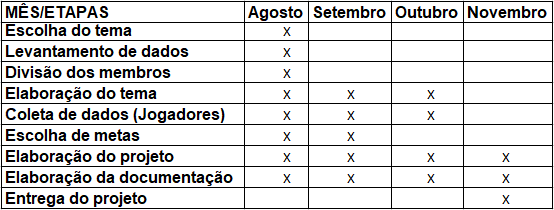
\includegraphics[scale=0.6]{Imagens/Cronograma.png}
        \caption{Cronograma do Projeto}
    \end{figure}

    \newpage %%
    \section{Referências}
    \noindent
    PUC PR. Mercado De Jogos Digitais Cresce No Brasil E No Mundo. G1 Globo, 08/10/2018. Disponível em: \textless https://g1.globo.com/pr/parana/especial-publicitario/puc-pr/profissionais-do-amanha/noticia/2018/10/08/mercado-de-jogos-digitais-cresce-no-brasil-e-no-mundo.ghtml\textgreater. Acesso em: 15 Out. 2019. \\
    
    \noindent
    ITENS ‘COSMÉTICOS’ MOVIMENTAM CULTURA E ECONOMIA DOS JOGOS. E-Arena. Disponível em: \textless https://e-arena.com.br/itens-cosmeticos-movimentam-cultura-e-economia-dos-jogos/\textgreater. Acesso em: 14 Out. 2019. \\
    
    \noindent
    MERCADO DE SKINS DE CS:GO PODE MOVIMENTAR ATÉ 10 BILHÕES DE DÓLARES POR ANO. The Enemy. Disponível em:\textless https://www.theenemy.com.br/esports/csgo-mercado-skins-10-bilhoes-valores-precos\textgreater. Acesso em: 14 Out. 2019. \\
    
    \noindent
    NEWZOO ARTICLES. NewZoo. Disponível em: \textless https://newzoo.com/insights/articles/\textgreater. Acesso em: 15 Out. 2019. \\
    
    \noindent
    SETOR DE GAMES CRESCE ACIMA DA MÉDIA NO PAÍS, MAS É O 13º DO MUNDO. O Tempo. Disponível em: \textless https://www.otempo.com.br/economia/subscription-required-7.5927739?aId=1.2224441\textgreater. Acesso em: 15 Out. 2019. \\

\end{document}